\documentclass{article}
\usepackage[UTF8]{ctex}
\usepackage{amsmath,mathtools,geometry,fancyhdr,tikz}
\geometry{a4paper,scale=0.7}
\pagenumbering{arabic}
\pagestyle{fancy}
\fancyhead[L]{励志AQ班}
\fancyhead[R]{每日一题(8.2)答案}
\fancyfoot[C]{\thepage}
\title{每日一题(8.2)答案}
\author{选题:门宇翎、李东宸\\答案制作:程昊一}

\begin{document}
\maketitle
\textbf{1.}{\kaishu 
若$x$, $y$均为实数, 且满足方程
\[x^2+y^2+4x-6y+13=0,\]
求$x+2y$的值.\\
(李东宸供题)}\\
\paragraph{分析}这个方程有两个未知数, 而且未知数\textbf{不是}整数, 所以尝试用配方以及平方式的非负性解决.
\paragraph{解}原方程等价于
\[(x^2+4x+4)+(y^2-6y+9)=0,\]
即
\[(x+2)^2+(y-3)^2=0.\]
\par 由于平方式的非负性, 得知
\[\begin{cases}
	x+2=0;\\y-3=0.
\end{cases}\]
即
\[\begin{cases}
	x=-2;\\y=3.
\end{cases}\]

\par\textbf{2.}{\kaishu 
某会议共有30名议员, 每两个人之间互相的关系为朋友或政敌. 每个人都有且仅有6个政敌. 每3个人组成一个委员会. 若一个委员会内的三个人的关系均为朋友或政敌, 则称这个委员会为“好委员会”. 求“好委员会”的数量. \\
(门宇翎供题)}

\paragraph{分析}对于这样的问题, 我们一般将整个结构抽象成节点和线段. 例如, 在这道题中, 我们将议员看做点, 若两个议员之间为朋友关系, 就将这两个点之间连上蓝色的线段; 反之则连接红色线段. 
\par 我们再来考虑“好委员会”在这个结构中代表什么. 显然, 如果三个点(议员)构成“好委员会”, 那么以这三个点为顶点的三角形的三条边应该是同色的, 我们称之为\textbf{同色三角形}, 如图\ref{fig:sameclrdelta}所示. 如果三个人不构成“好委员会”, 那么对应的三角形三边应该是不同色的, 我们称之为\textbf{异色三角形}, 如图\ref{fig:diffclrdelta}所示.  
\begin{figure}[htbp]%同色三角形,异色三角形
	\begin{minipage}{0.48\textwidth}
		\centering
		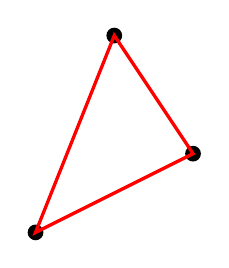
\begin{tikzpicture}
			\fill (0,0) circle(0.1);
			\fill (2,1) circle(0.1);
			\fill (1,2.5) circle(0.1);
			\draw [color=red,very thick] (0,0)--(2,1)--(1,2.5)--cycle;
		\end{tikzpicture}
		\caption{同色三角形}
		\label{fig:sameclrdelta}
	\end{minipage}
	\begin{minipage}{0.48\textwidth}
		\centering
		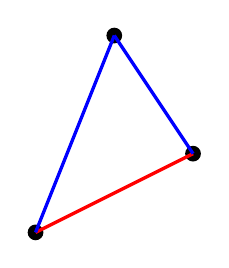
\begin{tikzpicture}
			\fill (0,0) circle(0.1);
			\fill (2,1) circle(0.1);
			\fill (1,2.5) circle(0.1);
			\draw [color=red,very thick] (0,0)--(2,1);
			\draw [color=blue,very thick] (1,2.5)--(2,1);
			\draw [color=blue,very thick] (0,0)--(1,2.5);
		\end{tikzpicture}
		\caption{异色三角形}
		\label{fig:diffclrdelta}
	\end{minipage}
	
\end{figure}
\par 我们再去考虑从哪方面下手.我们可以设同色三角形的个数为$x$, 异色三角形的个数为$y$, 这样我们得到了第一个方程: 
\[x+y=(\text{三角形的总个数})=\mathrm{C}^3_{30}. 
\footnote{这里的$\mathrm{C}^3_{30}$是指从30个物体中随意挑选3个物体的方法总数, 在题目中的意义就是随意挑选3个议员的方法数, 即三角形的个数. 一般地, $\mathrm{C}^n_m$表示从$m$个物体中随意挑选$n$个物体的方法的总数($m\ge n$).}
\]
\par 我们要想办法找到第二个方程. 事实上, 处理这种图论问题时, 我们有一个思想: \textbf{对}. 即如果我们的基本对象为点, 那么我们可以尝试分析“点对”, 即“边(线段)”; 如果我们研究的是边(线段), 那么我们可以考虑“边对”, 即“角”.
\par 在这里, 我们研究角, \textbf{同色角}(如图\ref{fig:sameclrangle}所示)与\textbf{异色角}(如图\ref{fig:diffclrangle}所示). 
\begin{figure}[htbp]%同色角,异色角
	\begin{minipage}{0.5\textwidth}
		\centering
		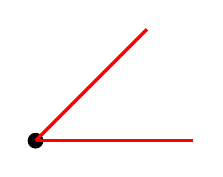
\begin{tikzpicture}
			\fill (0,0) circle(0.1);
			\draw [color=red,very thick](0,0)--(2,0);
			\draw [color=red,very thick](0,0)--(1.414,1.414);
		\end{tikzpicture}
		\caption{同色角}
		\label{fig:sameclrangle}
	\end{minipage}
	\begin{minipage}{0.5\textwidth}
		\centering
		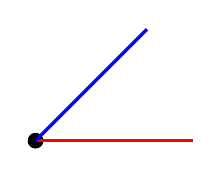
\begin{tikzpicture}
			\fill (0,0) circle(0.1);
			\draw [color=red,very thick](0,0)--(2,0);
			\draw [color=blue,very thick](0,0)--(1.414,1.414);
		\end{tikzpicture}
		\caption{异色角}
		\label{fig:diffclrangle}
	\end{minipage}
\end{figure}
\par 很显然, 每一个同色三角形提供3个同色角, 每一个异色三角形提供1个同色角. 那么, 同色角的总个数应该是$3x+y$. 另一方面, 对每一个顶点来说, 同色角的个数为$\mathrm{C}_{23}^2$(蓝色同色角个数)$+\mathrm{C}_6^2$(红色同色角个数), 即268个. 所以, 同色角共有$268\times30$, 即8040个. 
\par 那么, 我们就找到了第二个方程: 
\[3x+y=8040.\]
\par 然后, 解方程就是了.
\par 还有一个问题: 为什么不用考虑异色角? 你可以尝试一下, 最后会发现所列出来的方程可以由我们已经得到的两个方程推出.
\par 我们把过程书写一遍:
\paragraph{解}将议员看做点, 若两个议员之间为朋友关系, 就将这两个点之间连上蓝色的线段; 反之则连接红色线段.
\par 在这个结构中, 设同色三角形有$x$个, 异色三角形有$y$个, 那么从三角形总数的角度, 下列方程成立:
\begin{equation}\label{equ:amont}
	x+y=\mathrm{C}_{30}^3=4060 ;
\end{equation}
从同色角的角度, 应有
\begin{equation}\label{equ:sameclr}
	3x+y=30\times(\mathrm{C}_{23}^2+\mathrm{C}_6^2)=8040 .
\end{equation}
\par 联立(\ref{equ:amont})与(\ref{equ:sameclr})得
\[\begin{cases}
	x=1990 ;\\y=2070 .
\end{cases}\]
\par 综上: “好委员会”的数量为1990.
\end{document}